\documentclass[a4paper, top=10mm]{article}
\usepackage[french]{babel}
%for writing from the top
\usepackage{fullpage}
%for math
\usepackage{amsmath}
\usepackage{mathrsfs}
\usepackage{amsthm}
%for images
\usepackage{graphicx}
%for color
\usepackage{xcolor}
\usepackage{amssymb}
\usepackage{hyperref}
%for title
\title{\textbf{\huge{Un dessin?}}}
\author{Enigme n\textsuperscript{o}5}
\date{20 Janvier 2024}

\newtheorem*{hint}{Astuce}

\addtolength{\voffset}{-2cm}
\addtolength{\textheight}{5cm}


\begin{document}
	\maketitle
	
	\large
	Les vrai professeurs de mathématiques ne dessinent pas comme tout le monde.
	Ils se limitent aux dessins formés d'une courbe lisse fermée.
	
	De plus, au lieu de tracer cette courbe, ils se contentent de donner une approximation via les fonctions "horloges" de la forme $r_k e^{2\pi i k a_k}$ pour quelques $r_k$, $a_k$, $k \in \mathbb{Z}$.
	La courbe a considérer est alors donnée par représentation graphique de la somme des fonction horloges $f: [0,1] \to \mathbb{C} \approx \mathbb{R}^2$ avec $$f(t) = \sum_{k} r_k e^{2\pi i k a_k}$$.
	
	Un professeur vous donne quelques coefficients de fonctions horloges:
	
	\vspace{1cm}
	\begin{flushleft}
		\begin{tabular}{|c|c|c|}
			\hline
			$k$ & $r_k$, & $a_k$\\
			\hline
			$-7$ & $12$, & $137$\\
			$-6$ & $9$, & $-24$\\
			$-5$ & $5$, & $175$\\
			$-4$ & $5$, & $14$\\
			$-3$ & $28$, & $-147$\\
			$-2$ & $23$, & $-128$\\
			$-1$ & $163$, & $-109$\\
			$1$ & $60$, & $-71$\\
			$2$ & $32$, & $128$\\
			$3$ & $31$, & $147$\\
			$4$ & $21$, & $-14$\\
			$5$ & $10$, & $-175$\\
			$6$ & $4$, & $24$\\
			$7$ & $9$, & $-137$\\
			\hline
		\end{tabular}
	\end{flushleft}
	
	\begin{flushright}
		\vspace{-240pt}
		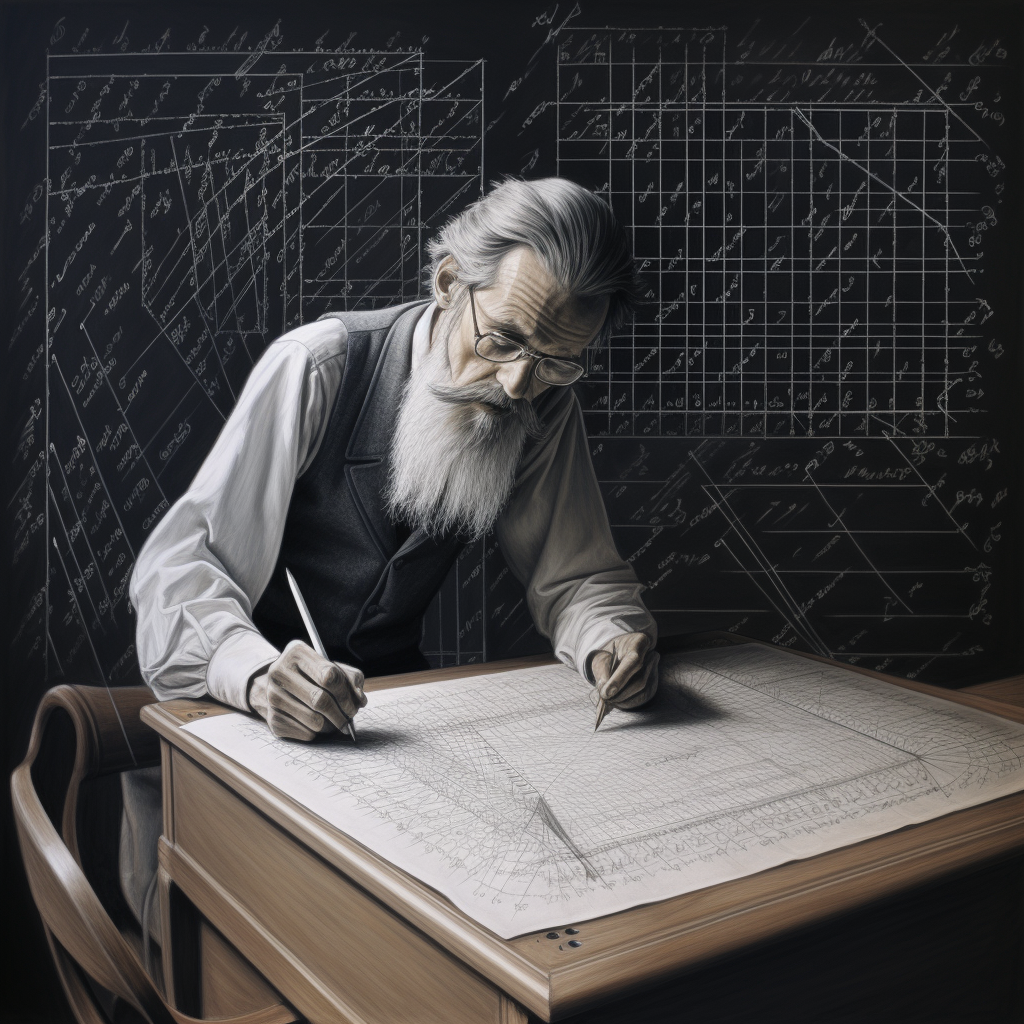
\includegraphics[width=250pt]{05mathematician_drawing.png}
	\end{flushright}

	{\Large \textbf{Qu'est-ce que le mathématicien a essayé de dessiné?}}
	\vspace{10pt}
	
	\begin{hint}
		Vous pouvez vous aider du site suivant:\\
		\url{https://pauldubois98.github.io/MathCurves/FourierCurves/}
	\end{hint}

	\begin{center}
		\vspace{5pt}
		
\includegraphics[height=150pt]{05QRcode.png}
	\end{center}
	
\end{document}